\documentclass[a4paper, 11pt]{article}
\usepackage{a4}
\usepackage[latin1]{inputenc}
\usepackage{listings}
\usepackage{verbatim}
\usepackage{epsf}
\usepackage[dvips]{graphicx}
\usepackage{rotating}

\lstset{
  language = c++, 
  breaklines = true,
  breakatwhitespace = true,
  showlines = true
}

\title{Openbus 1.5.0 - Architecture Description}
\author{Ma�ra Gatti}
\date{August 2010}

\begin{document}
\maketitle

\abstract{The Openbus is a CORBA-based Enterprise Service Bus. The goal of this document is to describe the Openbus 1.5.0 release architecture. It helps on the rationale for the architecture evolution and also helps new developers to understand Openbus mechanisms details. It is not the goal of this document to present Openbus motivation or SOA concepts.}

\section{Arquitecture Overview}

The Openbus is a component-based ESB and uses the SCS model and middleware. SCS \cite{SCS} stands for Software Component System. It comprehends both a component model and a distributed service-oriented middleware, being inspired primarily by CCM and COM \cite{COM}. The Openbus goal is to provide support for component-based application integration on complex, distributed, multi-language and multi-platform scenarios. Applications that want to provide and publish their functionalities as services on the bus are granted access via certificate authentications, while clients that need to find and use such services authenticate via login and password.

Like a CCM component, a SCS component is a composition of facets and receptacles. Facets are exported interfaces, which represent services provided by the component. Similarly, receptacles are required interfaces, which represent the component's external dependencies. SCS components can then be composed together themselves to create more complex applications. This composition between components is materialized by connections between facets and receptacles that can be established at runtime. It is important to note that although facets can be called services in a SOA semantic, components can also be, because they often represent a group of tightly associated services.

The SCS model is language-independent and extensible. It specifies three basic facets available in every component, besides user-specified facets. These basic facets handle the complexities of life cycle (IComponent), connections (IReceptacles) and introspection (IMetaInterface). To allow for more adaptable components, the model doesn't impose any rules on the creation or destruction of facets and receptacles. At present, there are four implementations of the model: C++, Java, Lua and .NET/C sharp. SCS components developed in different languages interoperate through the CORBA middleware, which also provides remote communication.

The SCS middleware also provides services to support remote deployment and execution that are composed as a Deployment Infrastructure and an Execution Infrastructure. All services are components themselves and benefit from both model and middleware features. They support dynamic (re)configuration of components at runtime, including the management of deployment plans, remote installation, remote instantiation and component connections, among other features.

\section{Basic Mechanisms}

Before presenting the basic component-based services of which Openbus is composed, it is important to understand the basic mechanisms underline the provided basic services. There are four basic mechanisms described as following.

\subsection{Leasing Mechanism}

A \textit{lease} is a contract that gives its holder specified rights
over property for a limited period of time. If the lease is not renewed before expiring, the resource may become available.

Openbus uses the leasing mechanism in order to control the components access through the bus. Through the access control service, the component can get a credential associated to a lease. If the lease expires, the credential is no longer valid and the component has to get a new one. 

Therefore, the client is responsible for implementing or using an existent lease renewer in order to ensure its credential will never expire, unless there is a network fault or faults like these.

\subsection{Security and Authentication}

In order to consume a service offer registered in Openbus, the components must provide a credential in each request. This credential is given to the client at the time that it is authenticated through the access control service.

Openbus uses CORBA Interceptors as a basic mechanism to support security and authentication. At the server side, if the client did not send its credential attached to the \textit{service context}, the server interceptor will not be able to validate the credential and the request will be refused.

Therefore, client interceptors are responsible for automatically adding the client credential as a \textit{service context} while the server interceptors validate this credential whenever a request is done. This security mechanism is transparent to the service implementation. Moreover, throughout all the request inside Openbus, the credential is available and any necessary further validations can be done.

\subsection{Interfaces Management and Authorization}

Any component that will provide a service in the Openbus is a member. The services are available through facets. Openbus has a basic mechanism for managing and authorizing those facets. This management is both done through the access control service and the registry service.
 
The access control service has a facet with methods for registering the members systems in Openbus. This registry is based on the creation of the \textit{System} entity followed by the addition of its deployments. The \textit{Deployments} are the \textit{System} instances and they are the entities which really authenticates in Openbus and export interfaces (facets).

The \textit{Deployment} identification has to be the same of the credential and the certificates must be registered by the management interface otherwise the login will not be validated by the access control service even though having the certificate into the Openbus security directory. During the Openbus installation, all the Openbus basic services are registered and it can be started without concerns.

The registry service component has a facet which manages which services (its facets) can be exported by the \textit{deployments}. It is possible to grant or revoke the right to export interfaces. However, only previously registered interfaces can be grants which means that there is an interface registration allowed by the registry service (the repID).

The registry service uses the \textit{IMetaIterface} to get all the deployment interfaces at the registration time. Then it searches for the grants authorizations. It also validates the credential with the access control service.

Any information (such as to list deployments or to list authorizations) can be queried by any user, but only administrators can update them.

\subsection{Fault Tolerance}

In order to deliver Quality of Service (QoS), Openbus has a replication mechanism which makes it highly fault tolerant. Both the access control service and the registry service can be replicated and have a monitor. The component replica monitor runs at the same host that the component replica to be monitored. To each component replica, there is one monitor. From time to time (which can be specified by the administrator) the monitor checks if the replica is alive. The replica might not be alive because of communication failures or because it has reached an undesired state. In both cases, the monitor will:
\begin{itemize}
 \item kill the component replica (if it is in an undesired state);
 \item unplug the component replica from the receptacle;
 \item restart another component replica;
 \item plug the component replica into the receptacle.
\end{itemize}

Furthermore, if several component replicas exist, they will be connected to the adaptive receptacle. If the client requests a component from this receptacle, only failure-free component replicas references will be given. 

The Smart Component Proxy encapsulates the component replicas group with transparency: the client thinks that she is interacting with a single server component. It detects when a fault is raised by the requested leader server component replica and forwards the request to another one, if any available. The number of times that the Smart Component will try to forward the request while no replica is available can be defined by the administrator.

In our current solution the Smart Component Proxy contains a hash table that maps the service facets keys with their interfaces and node's address. Currently, if some of CORBA systems exceptions\footnote{\textit{NO\_RESPONSE, COMM\_FAILURE, OBJECT\_NOT\_EXIST, TRANSIENT, TIMEOUT, NO\_RESOURCES, FREE\_MEM, NO\_MEMORY, INTERNAL.}} are raised, the Smart Component will fetch another replica.

The Smart Component can also be set by the administrator with regard to how many times it fetches a replica, how many time it waits for a reply, and how many time it waits between a fail reply and to fetch another replica. All those configurations can be externally updated during execution time, increasing adaptation.

Portable Interceptors do the same work that a Smart Component do: the client thinks that she is interacting with a single server component. The main difference between both is that there is a Smart Component to each dependable component. While there is only one interceptor to all dependable components and the interceptor has the reference to all the replicas in the group of each component. 

ACS and Registry Service components also have specific adaptive receptacle facets specialization in order to implement replica state synchronization according to one of the presented protocols with regard to the receptacle connections synchronization. 

The ACS Adaptive Receptacle implementation uses the multicast protocol to update the state if a successful connection or disconnection is done. Which means that each component replica will be invoked at the end of the request. The same behavior was implemented on the Registry Service Adaptive Receptacle.

During the Registry Service startup, it tries to connect to the ACS Adaptive Receptacle, therefore, all the active ACS component replicas will also receive this connection (if they are not already connected). In the case of the ACS startup, it will get all the connections of all active ACS component replicas and do a local connection, which means not activating the replication mechanism to avoid deadlocks.

The Registry Service component replicas access ACS Smart Component operations, rather than an ACS component replica stub and any faulty request will be transparently handled and redirected to an available ACS component replica. The ACS is not a receptacle of Registry Service because of the security design constrains set in the bus.

With regard to the compulsive leadercast protocol, all the ACS login operations (login by password, by certificate or by credential) activate the replication state using that protocol. They are the only operations which we decided to use this behavior since the credential generated by those operations is used all the time by the bus. On the other hand, we implemented the activation of this protocol as a dynamic policy: at any time the administrator can add or remove operations that activate the compulsive leadercast protocol.

On the other hand, in order to synchronize the credentials and offers between the ACS and Registry Service replicas, respectively, we use the non compulsive leadercast. Which means that unless there is a miss in any credential validation or offer's search, those data will not be synchronized.

Finally, all the clients that use the bus client library developed in Lua use Smart Components when they need a reference to the ACS component. We developed this feature through the Oil 0.5 \cite{oil05} \cite{oil10} facilities. While all the clients that use the bus client library developed in Java and C++ use our solution with Portable Interpcetors (those libraries use JacORB 2.3.0 \cite{jacorb}, Orbix 6.3 sp3 \cite{orbix} and MICO 2.3.13 \cite{mico}). In both cases they need to set the ACS component replicas host addresses in a configuration file and the fault manager iterative and cyclic searches for healthy replicas when a request fails. The administrator may specify how many times the fault manager is allowed to iterate over the replicas list.

\section{Basic Component-based Services}

The two basic component-based services that Openbus provides in order to implement the basic mechanisms described are the Access Control Service Component and the Registry Service Component.

\begin{figure} [htb]
\centering
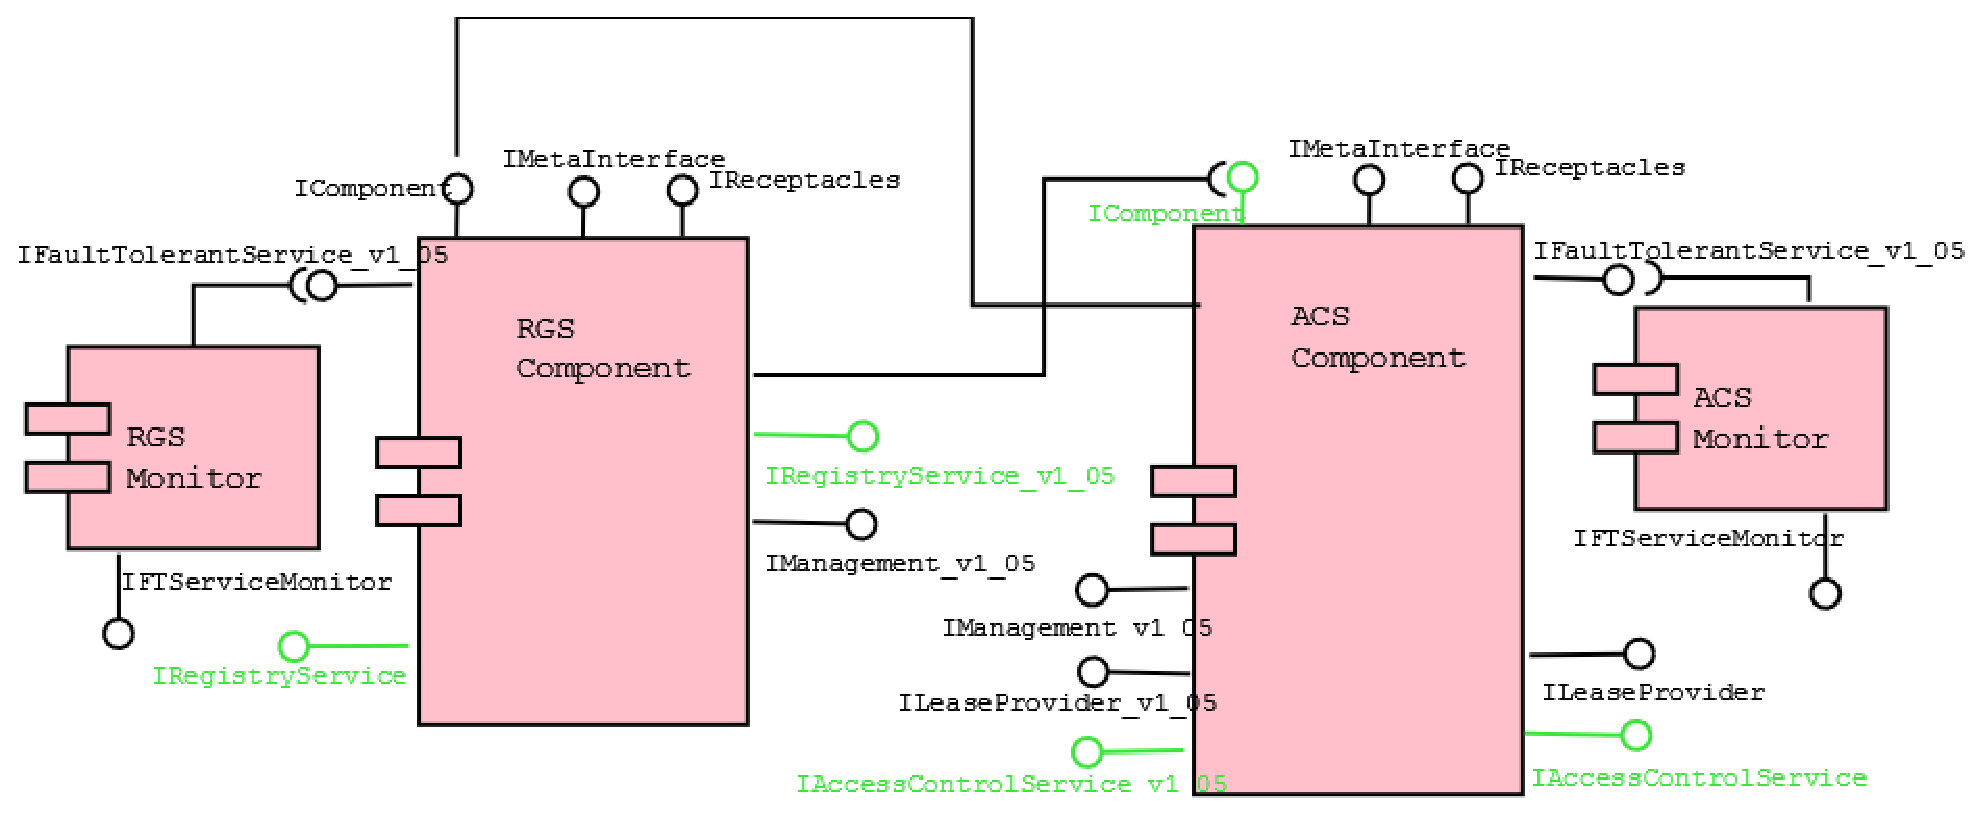
\includegraphics[width=14cm]{acs-rs.eps} %height=3in, 
\caption{Components Diagram: Access Control Service Component and Registry Service Component. The green facets are the ones used by (or visible for) the clients.}
\label{fig:acs-rgs}
\end{figure}

From figure \ref{fig:acs-rgs}, it is possible to see all the components facets, dependencies, and relationships. Both the Access Control Service Component and the Registry Service Component are SCS Components, therefore they have three facets in common: \textit{IComponent}, \textit{IMetaInterface} and \textit{IReceptacles}.

Moreover, the both components have two kind of facets, the ones which provide Openbus 1.4.x release services and the ones which provide Openbus 1.5.x release services. There are two new facets (they didn't exist in Openbus 1.4.x release) which are the \textit{IManagement\_v1\_05} and \textit{IFaultTolerantService\_v1\_05}. Although they are new, they are also tagged with the Openbus version's number because from  Openbus 1.5.0 release, any interface must be tagged with the Openbus version's number. This is a requirement in order to: i) make it clear that this interface didn't exist before to any new or old clients, and also ii)  make it a distribution pattern.

Another new improvement implemented in Openbus with regard to its previous version is that the Access Control Service Component has a receptacle for the Registry Service Component and vice-versa. Both receptacles are adaptive as further described in this document.

Finally, figure \ref{fig:acs-rgs} also illustrates two new components in Openbus: the monitors. They are not visible to the clients and only exist to increase dependability. Their mechanisms were explained in section 2.4, when we described the fault tolerant basic mechanisms implemented in Openbus and the fault tolerance conceptual model is also further described in this document.

\subsection{Access Control Service Component} 

The Access Control Service Component is the Openbus entry point. All services have reference to it and through the \textit{IComponent} facet, the \textit{ILeaseProvider} and \textit{IAccessControlService} facets can be retrieved.

In order to an user (clients or servers) to login in the bus to consume or provide services, it is necessary to authenticate to get a credential (that provides access in the bus). The authentication can be done by providing an user name and password or a digital certificate. Clients applications usually use the former and server applications usually use the latter.

After the authentication, a credential is generated and given to the user. This credential is composed by an unique identification and by the entity name of which this credential is associated (which can be an user or service). This credential has a life cycle and must be renewed before expiring.

\subsubsection{Conceptual Model of the Basic Entities}

Figure \ref{fig:acs} illustrates the conceptual model of the basic entities of the Access Control Service Component. It is mainly composed by the facets that implements the \textit{IAccessControlService} interfaces (both versions), the relationship with the \textit{IManagement\_v1\_05} interface (and facet), the credential related entities, and finally the lease related entities.

\begin{figure} [htb]
\centering
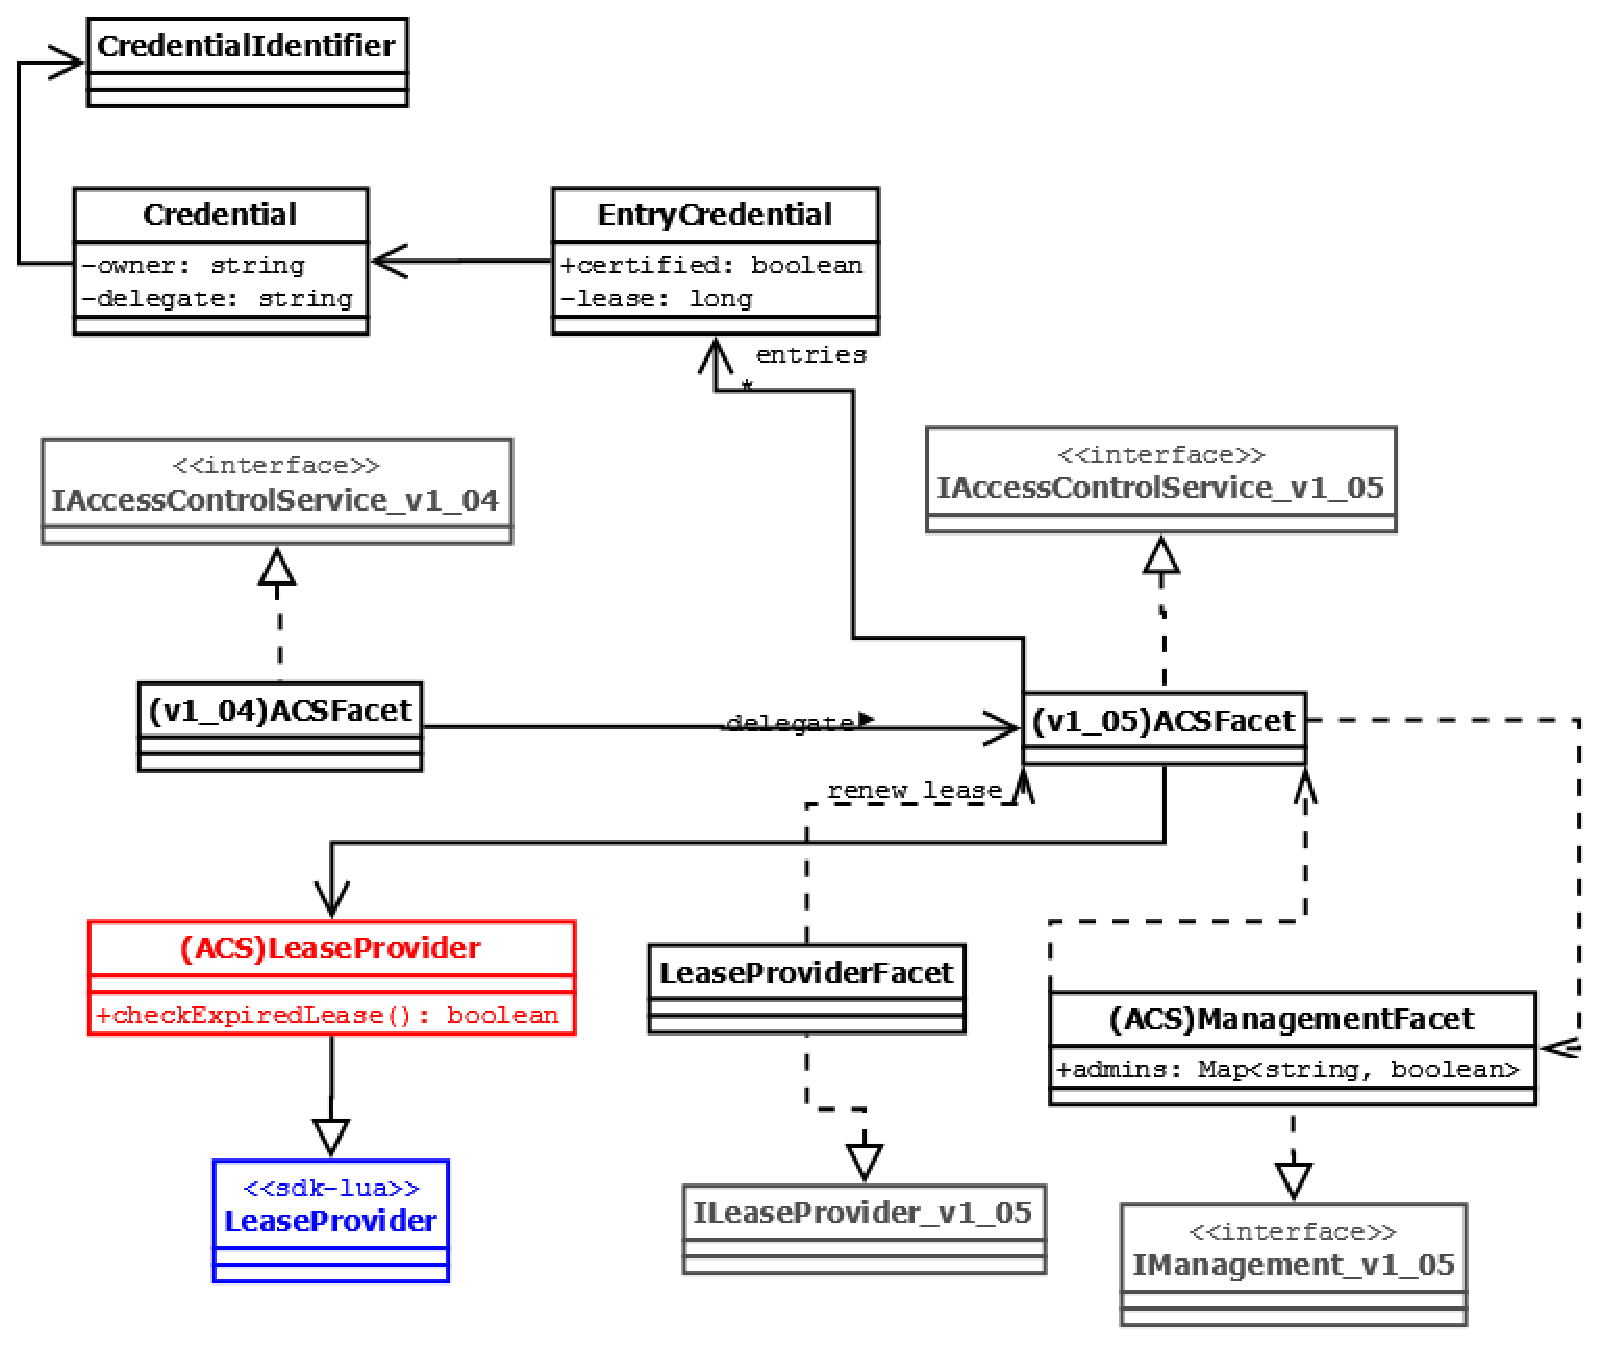
\includegraphics[width=10cm]{acs.eps} %height=3in, 
\caption{Access Control Service Component: Conceptual Model of the Basic Entities}
\label{fig:acs}
\end{figure}

Let's start with the credential related entities. The IDL defines three basic entities: the \textit{CredentialIdentifier}, the \textit{Credential} and the \textit{EntryCredential}. The \textit{CredentialIdentifier} and \textit{Credential} previously were in the Openbus 1.4.x release, but the \textit{EntryCredential} was added in the Openbus 1.5.0 release. The  \textit{CredentialIdentifier} just provides the unique identification for each credential, while the \textit{Credential} describes the structure that the user receives when login in the Openbus. The \textit{EntryCredential} on the other hand are structures exchanged between the Access Control Service Component replicas during state synchronization and have more information such as if the credential is certified (was generated because of a login by certificate) and the lease time (for how long it is valid). The \textit{ACSFacet} has a list of credentials entries.

For illustrative purposes, we put the number of the Openbus release version in front of the \textit{ACSFacet} names. As it is illustrated, the implementation of the \textit{IAcessControlService} delegates its behavior to the new \textit{ACSFacet} (the implementation of the \textit{IAccessControlSevice\_v1\_05}).

Because the Access Control Service Component provides a facet to behavior as a lease provider, called the \textit{LeaseProviderFacet}, this in turn depends on the \textit{ACSFacet} in order to renew the credentials' lease. The \textit{ACSFacet} also uses the \textit{LeaseProvider} (class provided by the sdk-lua) and implements the \textit{checkExpiredLease()} method of this class. We illustrated this polymorphism in the conceptual model through the \textit{(ACS)LeaseProvider} class which currently does not exist in Openbus 1.5.x release.

Finally, the \textit{ACSFacet} depends on the \textit{ManagementFacet} (illustrated as \textit{(ACS)ManagementFacet} in order to differentiate from the one implemented in the Registry Service Component) when checking for permissions and the \textit{ManagementFacet} also depends on the \textit{ACSFacet} when consulting the credentials entries.


\subsection{Registry Service Component} 

This component is responsible for controlling all the service offers available in the Openbus. Any component that needs to offer a service must register its offer explicitly in the Registry Service Component. The components that need to use a service can get the service providers localization and their properties through the registry service queries.

\subsubsection{Conceptual Model of the Basic Entities}

Figure \ref{fig:rgs} illustrates the conceptual model of the entities and related entities that the basic behavior of the Registry Service Component depends on.

To start with, the \textit{RSComponent} class represents the implementation of the \textit{IComponent} interface implementation. At the \textit{startup} method, the Registry Service locates the Access Control Service Component through the \textit{Openbus} class (sdk-lua) and requests a login by certificate. Even if there is only one Access Control Service Component active replica, the Registry Service gets the Smart Component reference from the  \textit{Openbus} class and the \textit{IComponent} facet from the Access Control Service Component is connected to the Registry Service receptacle. At this time, the Access Control Service Component (more specifically, the \textit{connect} operation of the \textit{ACSReceptacle} facet) also connects the Registry Service \textit{IComponent} facet in its receptacle.

Each service offer is represented by the \textit{ServiceOffer} entity. The services (both clients or servers) only manipulate this element. When a server application wants to provide a service offer, it creates a service offer entry with this structure. The \textit{ServiceOffer} has also a reference to the service through the association to the service's \textit{IComponent} facet. The \textit{RSFacet} class has a list of \textit{ServiceOfferEntry} which represents a complete entry of the service offer. The Registry Service Component replicas use this complete structure to synchronize the replicas state with regard to the service offers. The \textit{ServiceOffer} class has the service offer properties definition as defined in the IDL. While the \textit{ServiceOfferEntry} has an index map of those properties in order to speed client queries. It also has an index map of the authorized interfaces related to the services that works as a cache mechanism. This is further explained in the Management Conceptual Model section.

\begin{figure} [htb]
\centering
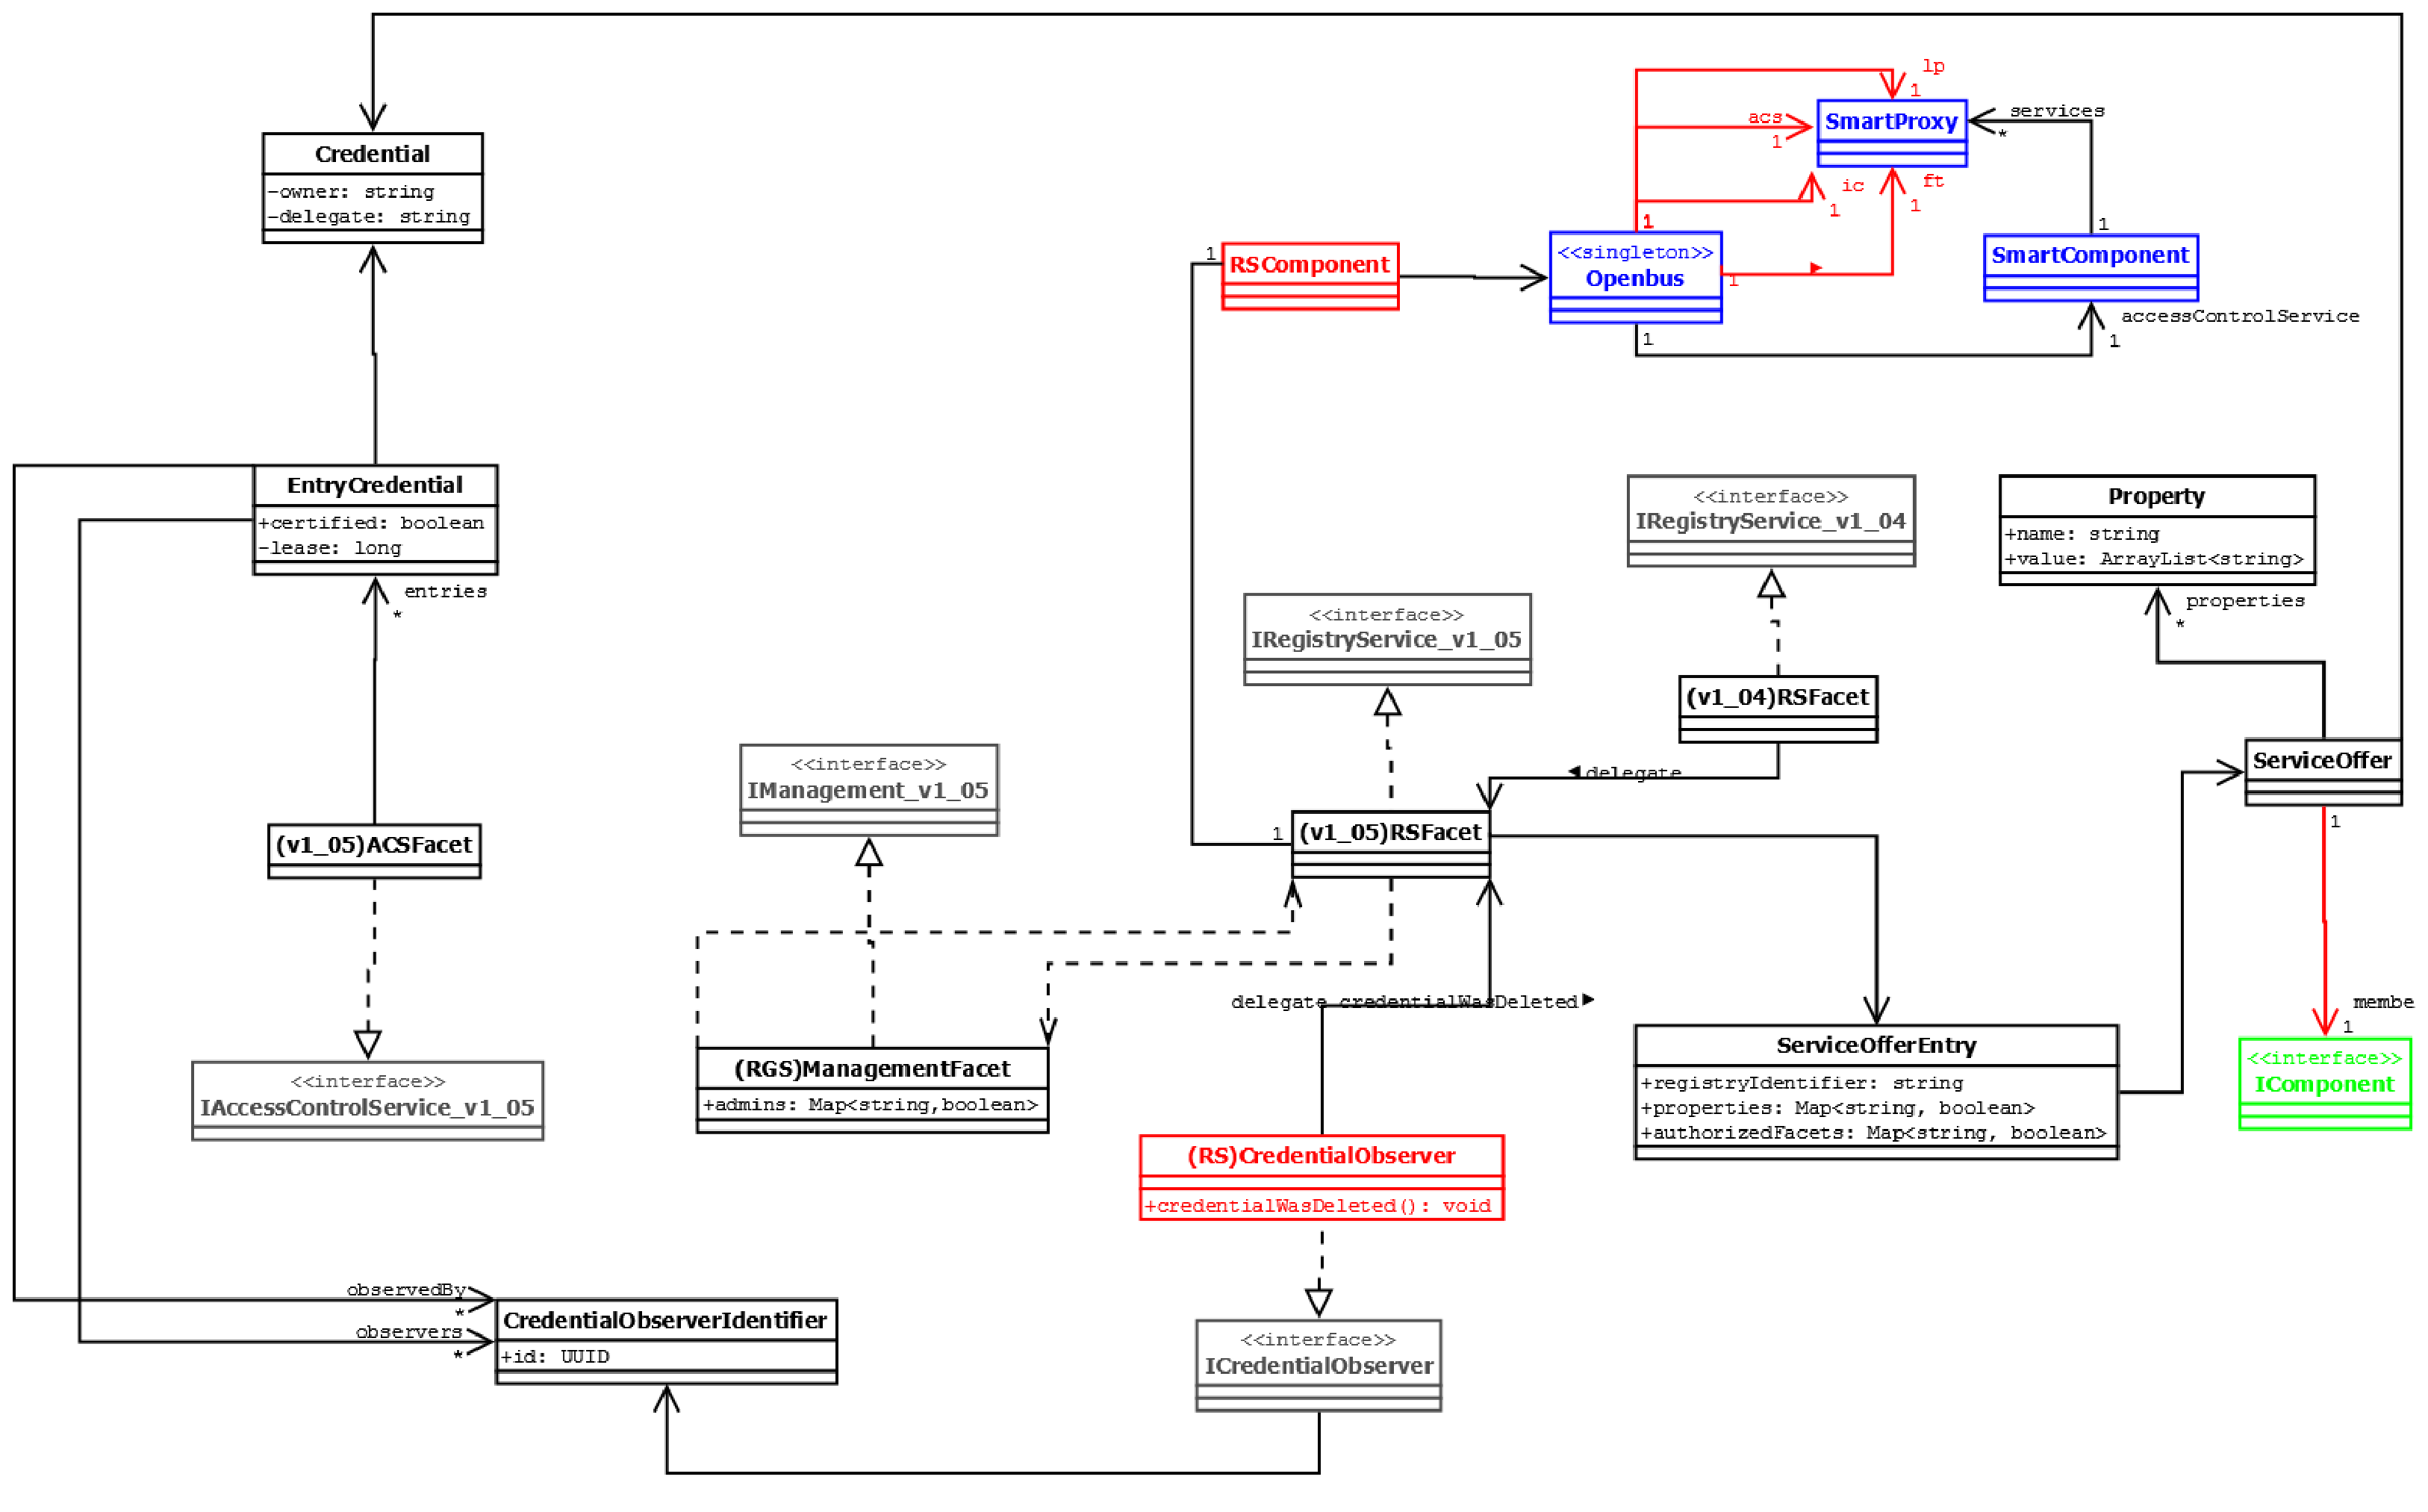
\includegraphics[width=14cm]{rgs.eps} %height=3in, 
\caption{Registry Service Component: Conceptual Model of the Basic Entities}
\label{fig:rgs}
\end{figure}

Just like explained for the Access Control Service Component, for illustrative purposes, we put the number of the Openbus release version in front of the \textit{RSFacet} names. As it is illustrated, the implementation of the \textit{IRegistryService} delegates its behavior to the new \textit{RSFacet} (the implementation of the \textit{IRegistrySevice\_v1\_05}).

Finally, the Openbus has a credential observer mechanism. The Registry Service Component implements \textit{credentialWasDeleted} method of the \textit{ICredentialObserver} interface. This behavior is illustrated through the \textit{(RS)CredentialObserver} class which in fact delegates this implementation to the \textit{RSFacet} class. The \textit{EntryCredential} class has a reference to all observers of the current credential entry. The \textit{EntryCredential} also as an index map of the observers for optimizations (illustrated by the \textit{observedBy} relationship).


\subsection{Management Conceptual Model}

As already described the Openbus has a basic mechanism for managing and authorizing those facets. This management is both done through the access control service and the registry service. 

\begin{figure} [htb]
\centering
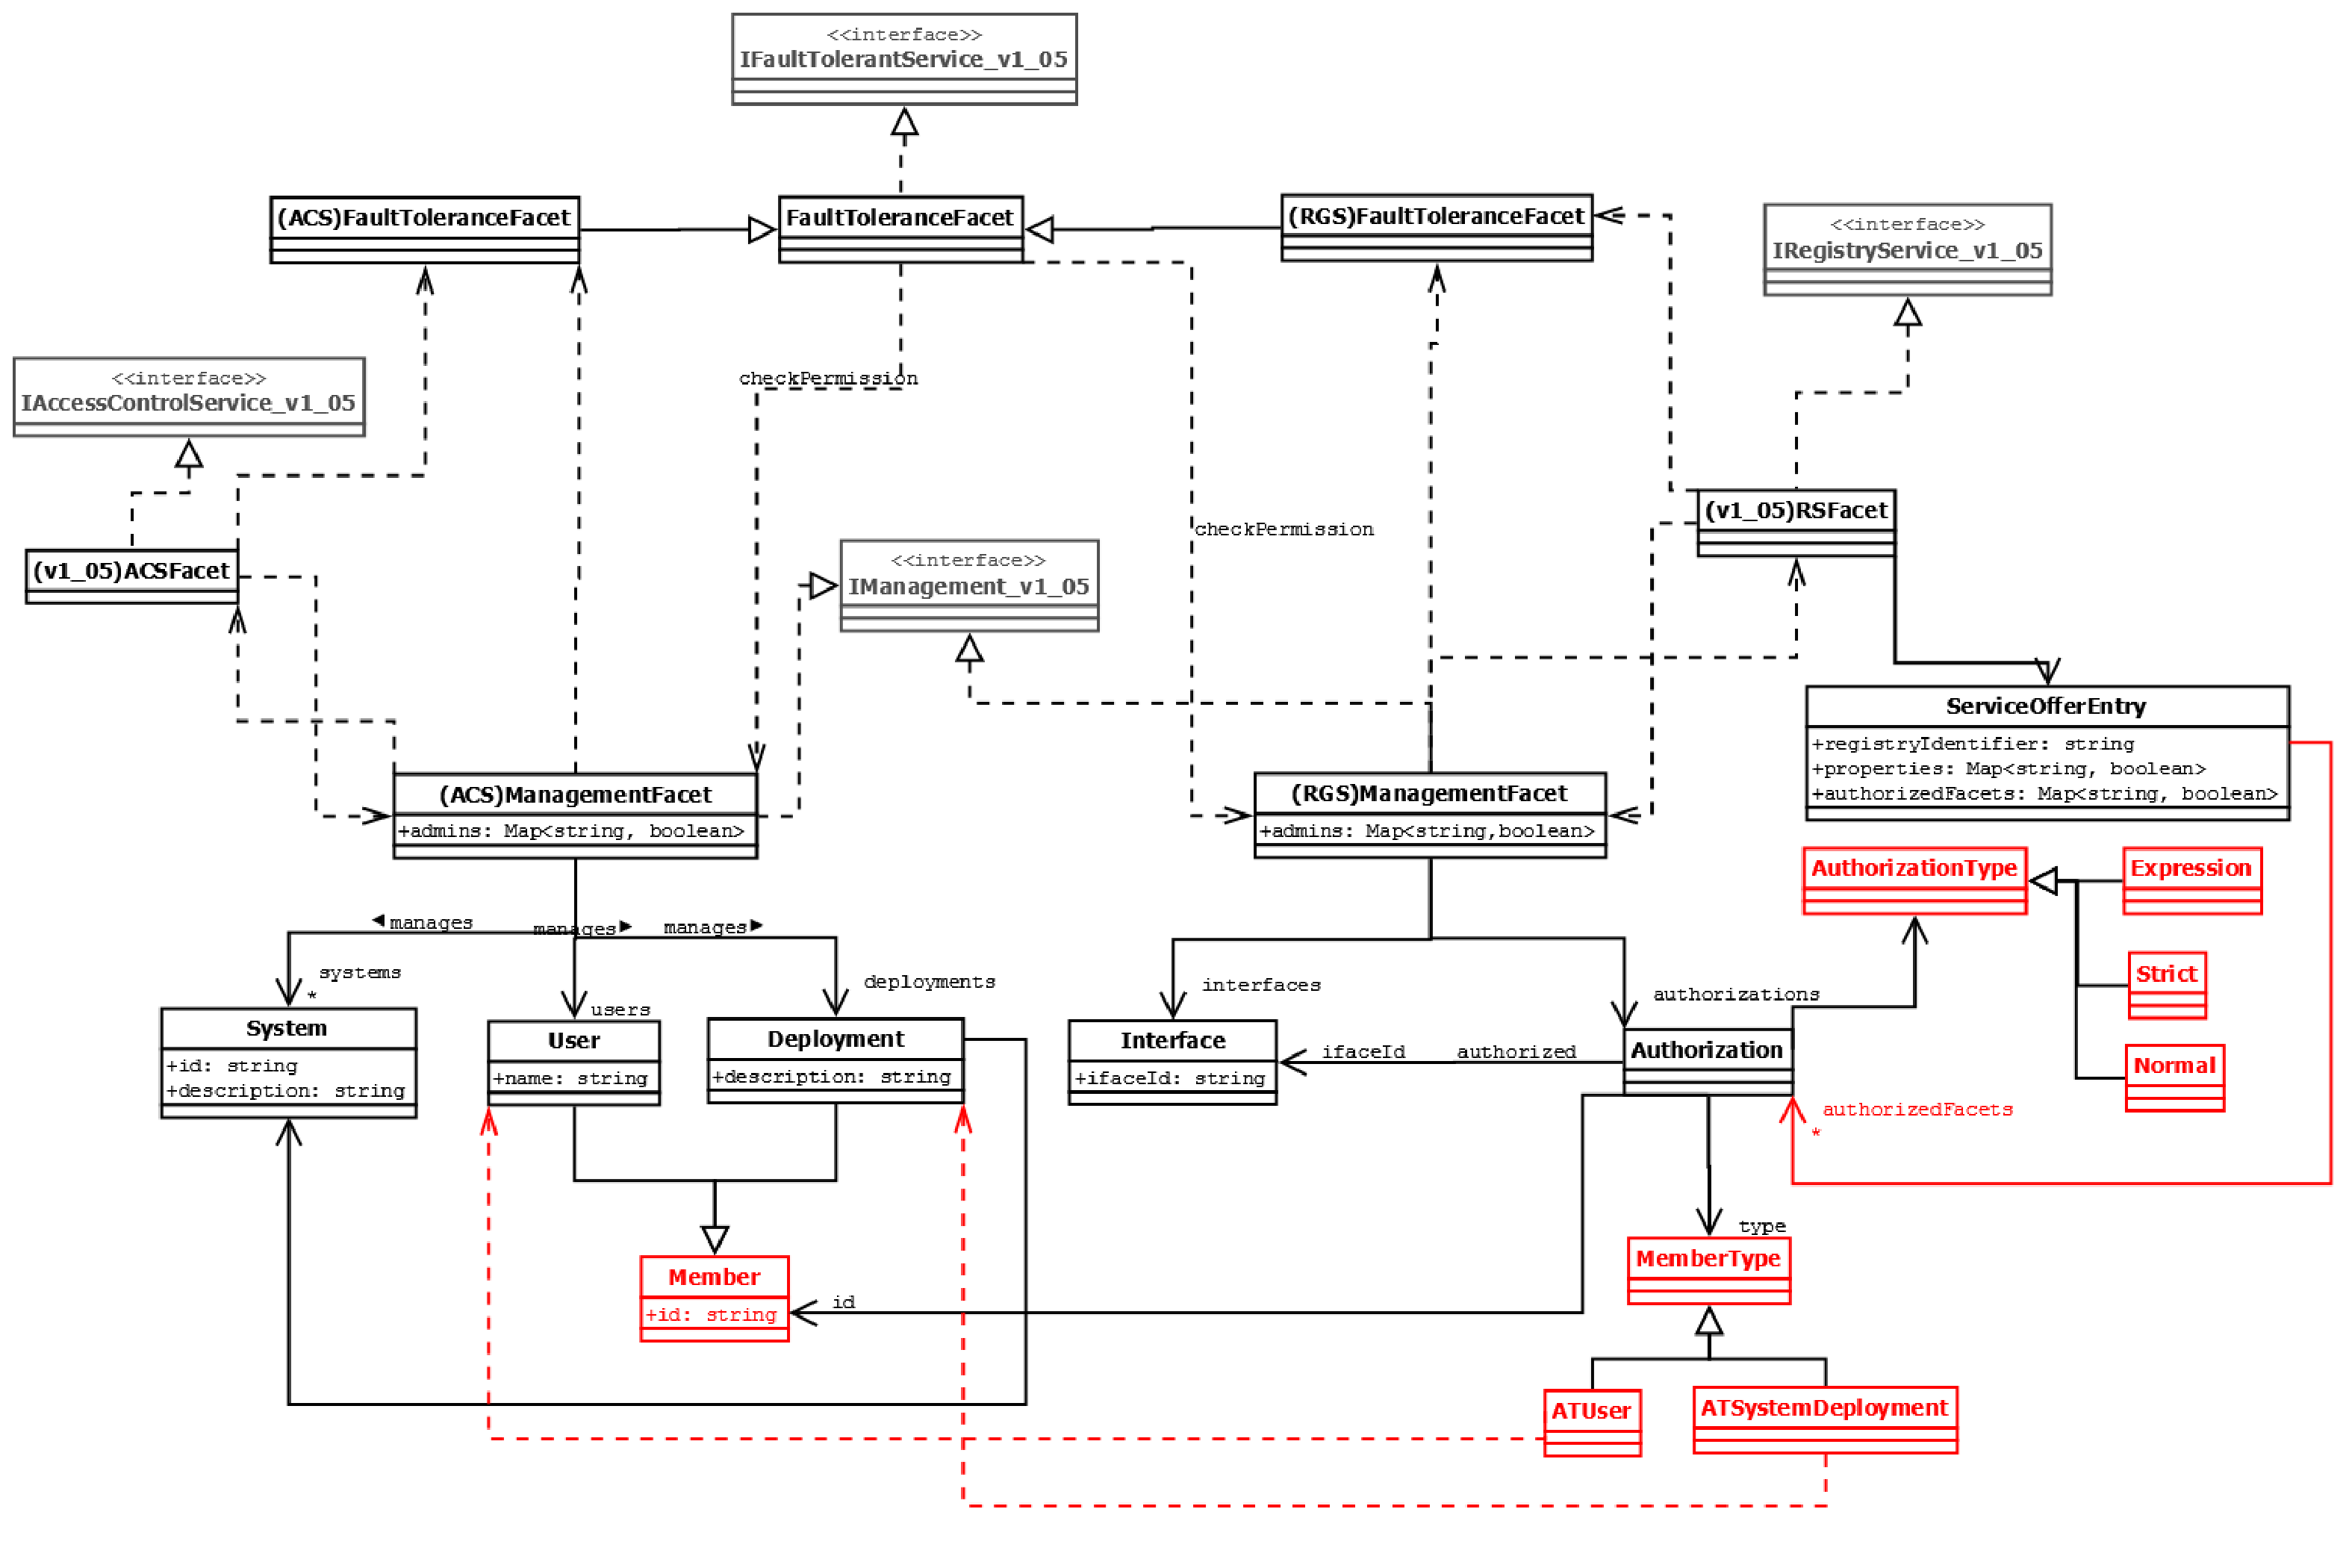
\includegraphics[width=14cm]{mgm.eps} %height=3in, 
\caption{Management Conceptual Model: an integrated overview}
\label{fig:mgm}
\end{figure}

The entities were already described before in this document, but in order to illustrate their relationships with the classes from the Access Control Service Component and the Registry Service Component figure \ref{fig:mgm} is presented.

The \textit{ManagementFacet} class of the Access Control Service Component implements the \textit{IManagement\_v1\_05} interface. This class has a map of strings and booleans which represents the administrators of the system. The \textit{ManagementFacet} class of Registry Service Component also has this map. The \textit{(ACS)ManagementFacet} class manages the \textit{System}, \textit{User} and \textit{Deployment}. There are two types of members: users (represented by the \textit{User} class) and system deployments (represented by the \textit{Deployment} class). 

When an authorization is added in Openbus through the \textit{(RS)ManagementFacet} class of the Registry Service Component, it is necessary to provide the identification of the \textit{Member} (a string in the code), and the \textit{Authorization} is saved according to the member type: \textit{User} or \textit{Deployment}, represented only illustrative by the \textit{ATUser} and \textit{ATSystemDeployment} classes - they are just strings in the \textit{type} attribute in the code. This type should not be misunderstood as the \textit{Authorization} type, which can be: an \textit{Expression}, \textit{Strict} or \textit{Normal}.

And finally, for optimizations purpose, the \textit{ServiceOffer} class has an index map of the authorized interfaces.

\subsection{Fault Tolerance Conceptual Model}

As already described, Openbus has a replication-based fault tolerant mechanism which increases Openbus QoS.

Figure \ref{fig:ft} illustrates the main entities and relationships of the fault tolerant mechanism in an integrated overview. Since both the Access Control Service Component and the Registry Service Component can be replicated, they have their monitors which are implemented by the \textit{FTACSMonitorFacet} and \textit{FTRSMonitorFacet}. They are implementations of the \textit{IFTServiceMonitor} interface describe in the IDL.

At the Access Control Service Component and Registry Service Component startup, the \textit{(ACS)FaultToleranceFacet} and the \textit{(RS)FaultToleranceFacet} are intialized, respectively. They extend the \textit{FaultToleranceFacet} class which implements the common behavior as an implementation of the \textit{IFaultTolerantService\_v1\_05} interface.

Because the \textit{(ACS)FaultToleranceFacet} update the \textit{ACSFacet} state, it depends on the \textit{EntryCredential}. The same occurs with the \textit{(RS)FaultToleranceFacet} with regard to the \textit{ServiceOfferEntry}. At the same time the \textit{ACSFacet} and the \textit{RSFacet} depend on their respectives fault tolerant facets in order to requesting for synchronization state if any data is missing.

Furthermore, the \textit{FaultToleranceFacet} depends on the \textit{ManagementFacet}s in order to check the permission of updating or killing a replica. At the same time the \textit{ManagementFacet} depends on the \textit{FaultToleranceFacet}s in order to request for synchronization state each time any Management operation is requested in Openbus and there are two or more active replicas.

\begin{figure} [htb]
\centering
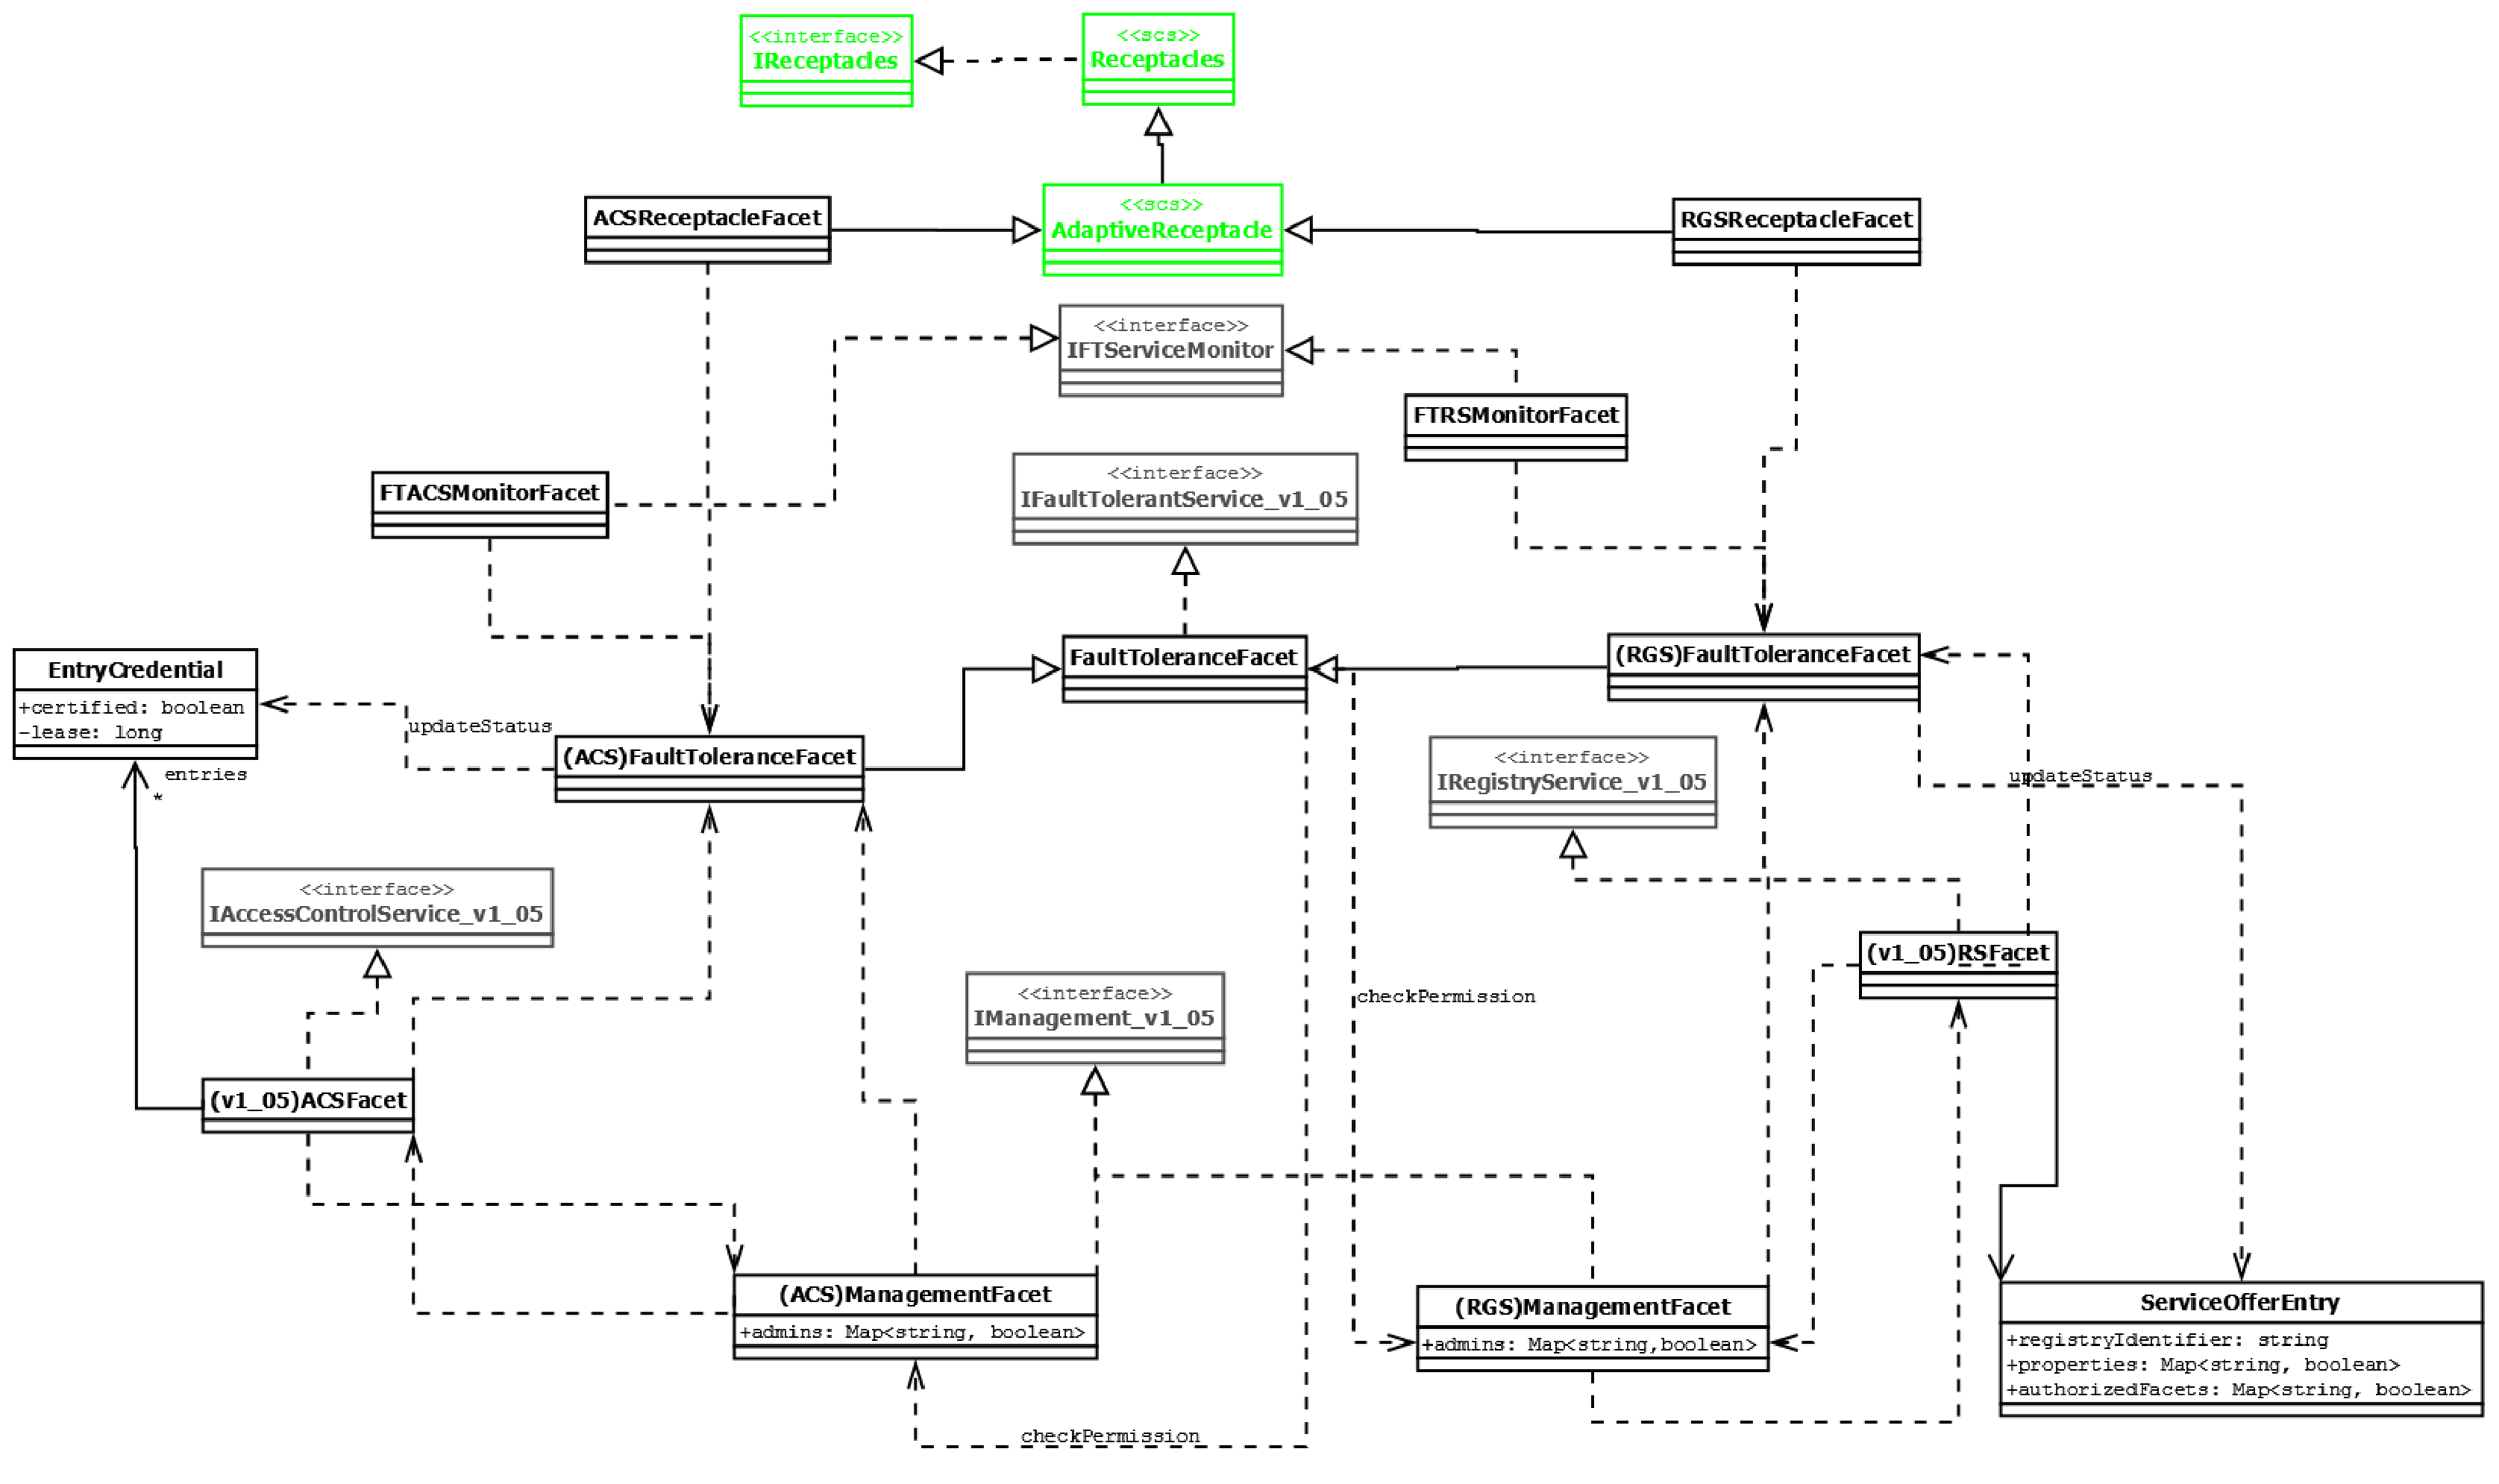
\includegraphics[width=14cm]{ft.eps} %height=3in, 
\caption{Fault Tolerance Conceptual Model: an integrated overview}
\label{fig:ft}
\end{figure}

Finally, the \textit{ACSReceptacleFacet} and the \textit{RGSReceptacleFacet} extends the \textit{AdaptiveReceptacles} class which is the implementation of an adaptive receptacles. This means that this receptacle always checks for available and reliable services before providing them through the \textit{getConnections()} operation. In other words, any time the client requests the reference to the Registry Service Component, the Access Control Service Component will only provide an available and reliable replica.

In each startup, both the Access Control Service Component and the Registry Service Component look for existent receptacles in their respective replicas. Which means that if there is any Registry Service Component connected to other Access Control Service replica, it will be connected to the current replica being started up. The same happens to the Registry Service Component. 

When a service is disconnected from the receptacle, the replicas also disconnect it from their receptacles.

\section{Session Service Component} 

There is also a third component, called Session Service Component that Openbus provides which helps on the information sharing between a group of clients.

\begin{figure} [htb]
\centering
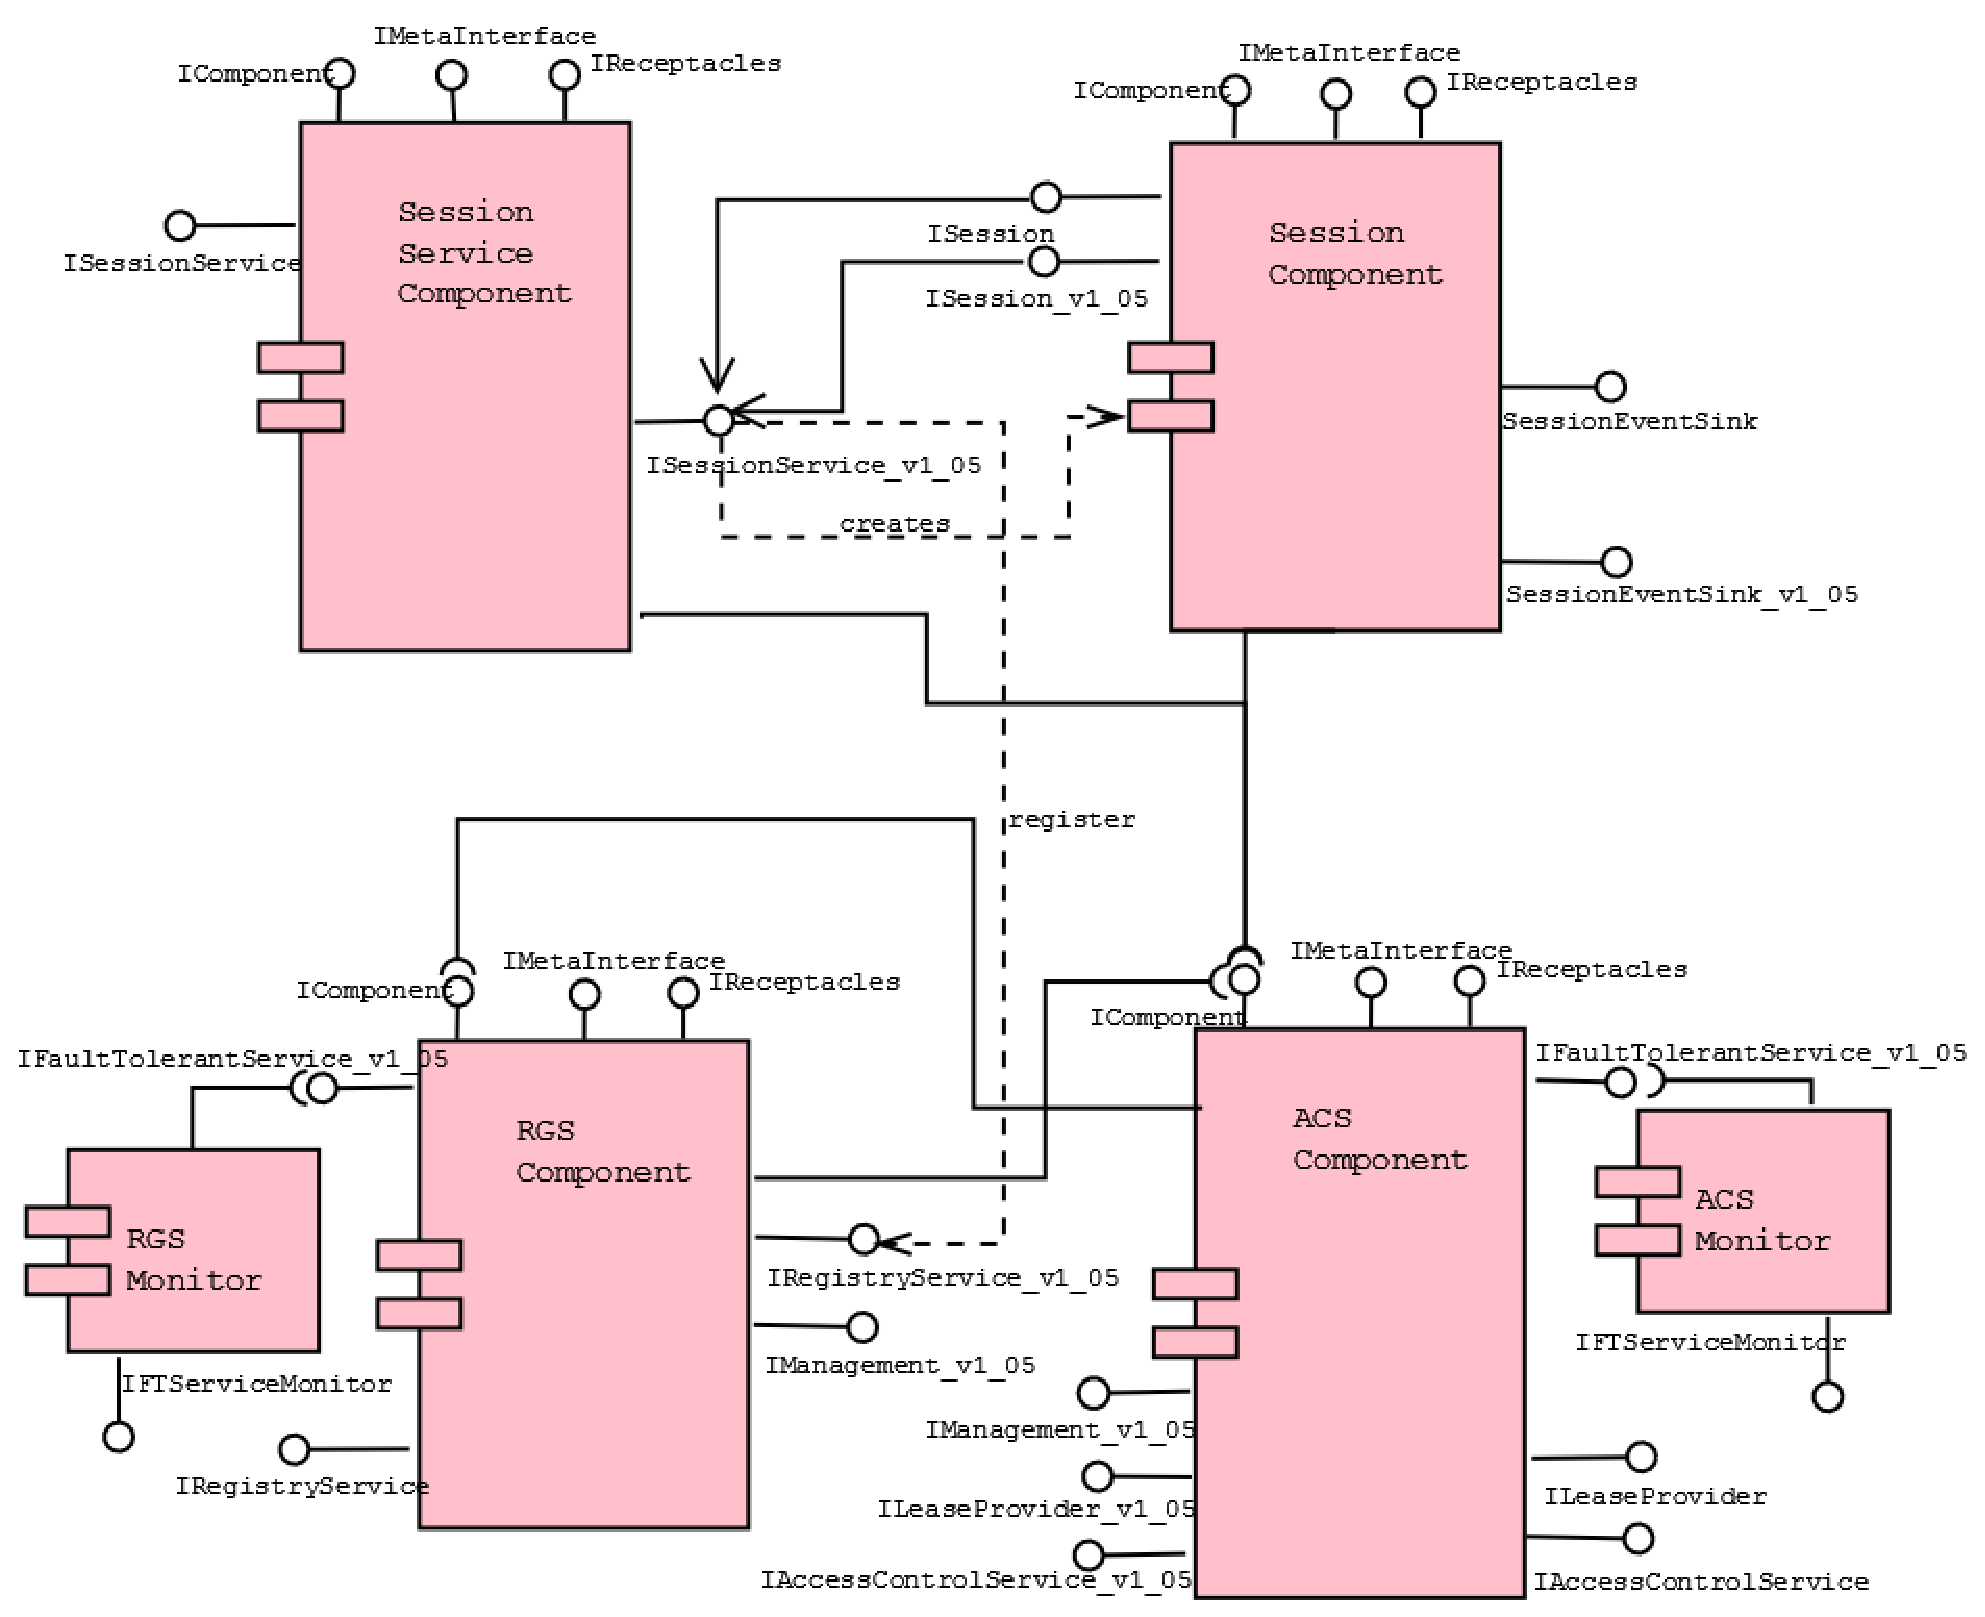
\includegraphics[width=14cm]{ss.eps} %height=3in, 
\caption{Session Service Components Diagram and Openbus Basic Components}
\label{fig:ss}
\end{figure}

As it is illustrated in figure \ref{fig:ss} the \textit{Session Service Component} and the \textit{Session Component} connect to the Access Control Service Component. The \textit{ISessionService\_v1\_05} interface is responsible for creating sessions and the \textit{SessionServiceComponent} facet (implementation of the \textit{IComponent} SCS interface) registers the \textit{ISessionService\_v1\_05} interface offers (and also the \textit{ISessionService} interface, from Openbus 1.4.x version release) into the Registry Service.

In figure \ref{fig:ss-classes} one can see in more details the Session Service elements and relationships. During the \textit{SessionServiceComponent} startup, first the properties for each session service interface are created. Then they are inserted as service offers and registered in the Registry Service (through the \textit{RSFacet}) so the clients can find them through the Registry Service. 

\begin{sidewaysfigure}
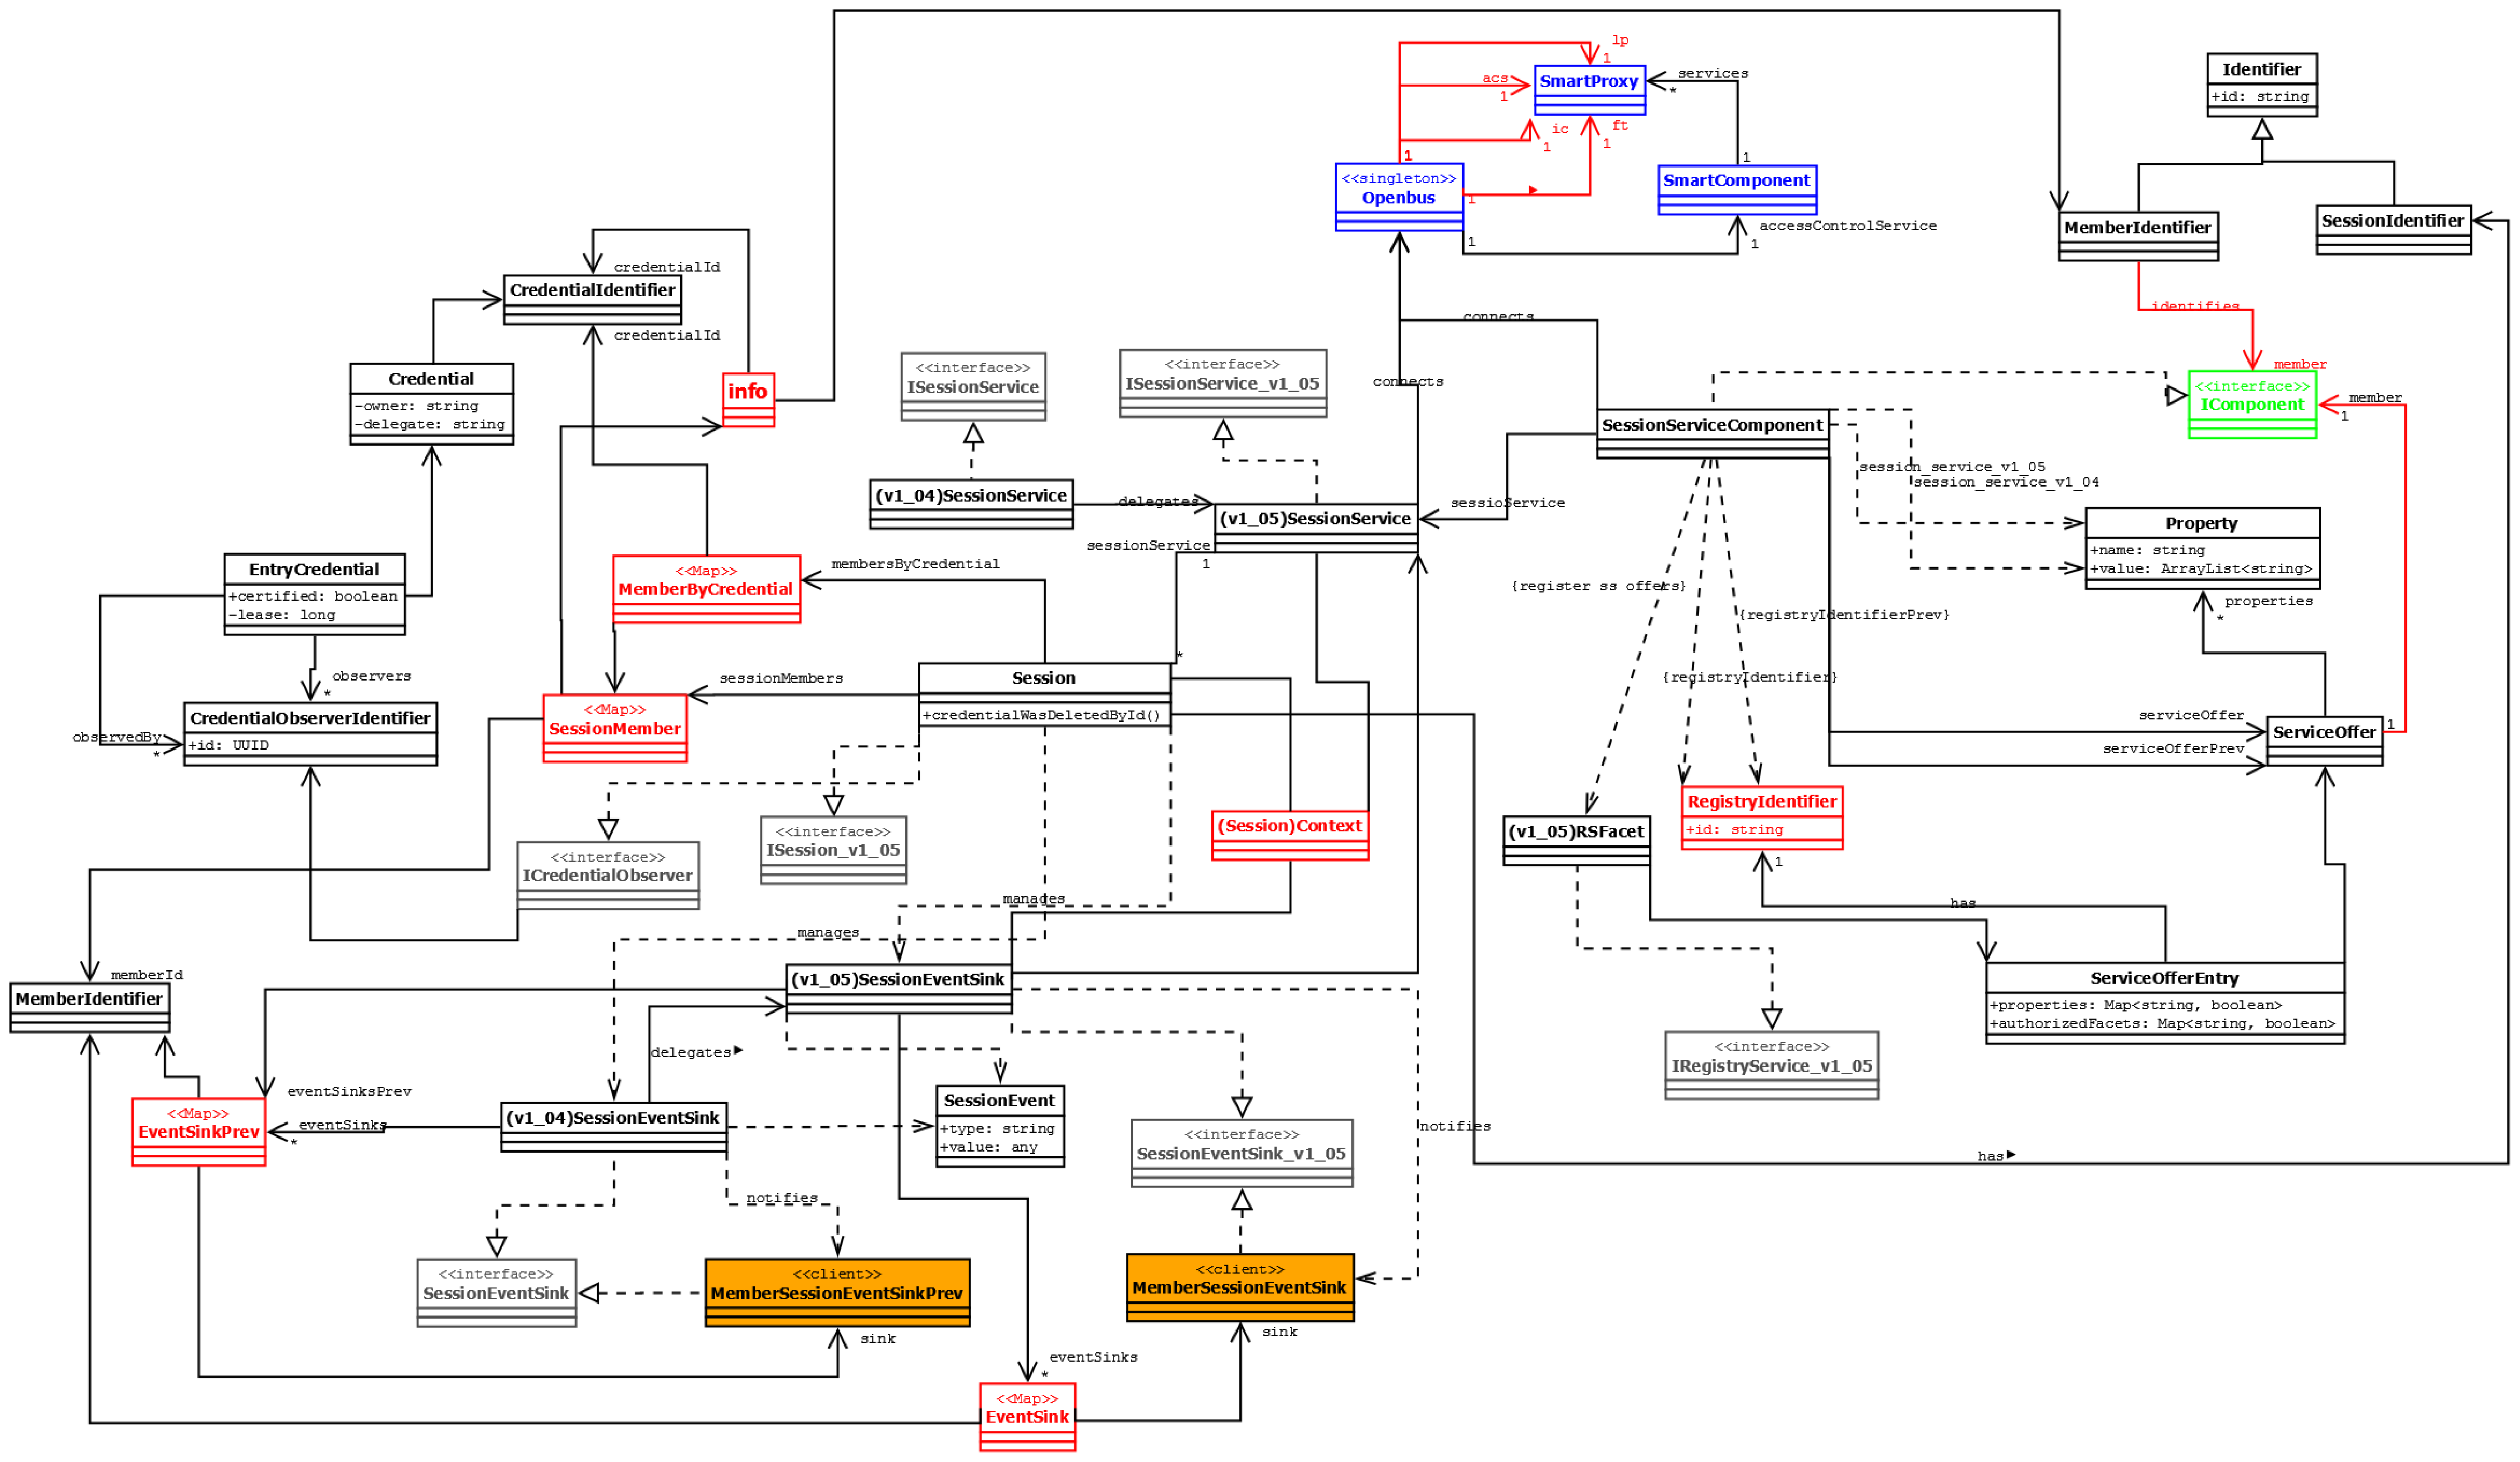
\includegraphics[height=18cm,width=24cm]{ss-classes.eps} %height=3in, 
\caption{Session Service Class Diagram - Conceptual Model}
\label{fig:ss-classes}
\end{sidewaysfigure}

Each \textit{SessionService} can have multiple \textit{Session}s. The \textit{Session} facet implements the \textit{ISession\_v1\_05} (or v1\_04, if the case) and the \textit{ICredentialObserver} interfaces. Which means that they are credential observers. The \textit{Session} facet has a list of session members which is a Map of \textit{info} indexed by the \textit{MemberIdentifier}. The \textit{info} class is a representation of a Lua table that contains the \textit{CredentialIdentifier} and \textit{MemberIdentifier}.

The \textit{Session} facet also has a list of members by credential (represented by the \textit{MemberByCredential} class), which is a Map of \textit{SessionMember} indexed by the \textit{CredentialIdentifier}.

The \textit{Session} facet manages the \textit{SessionEventSink} facets (both v1\_04 and v1\_05), which means that the former is responsinble for adding event sinks in their lists. An Event Sink is a service interface that will be implemented by the client. The information sharing works as follows: whenever a \textit{SessionEvent} in sent to the \textit{Session}, the \textit{SessionEventSink} facets (server) actively contacts one of more \textit{MemberSessionEventSink} (clients' implementation of the \textit{SessionEventSink} interface) in order to notify the former of specific events. This is done through the iteration of the \textit{eventSinks} list that the \textit{SessionEventSink} facet has. This list is a list of Maps that contain the \textit{MemberSessionEventSink} and is indexed by the \textit{MemberIdentifier}.


\begin{thebibliography}{50}
\bibitem[1]{Chappell}
Chappell, D. 2004 Enterprise Service Bus. O'Reilly Media, Inc.

\bibitem[2]{Szyperski1998}
Szyperski, C. Component Software: Beyond Object-Oriented Programming. ACM Press : Addison-Wesley Publishing Co. 1998.

\bibitem[3]{EJB}
Sun Microsystems. Enterprise JavaBeans Specification. v3.0. http://java.sun.com/ejb/

\bibitem[4]{OMG2004}
OMG. CORBA Components. OMG Document formal/04-03-01 (CORBA, v3.0.3). 2004. http://www.omg.org

\bibitem[5]{DotNet}
Microsoft. Overview of the .NET Framework 4. http://msdn.microsoft.com/en-us/library/a4t23ktk.aspx

\bibitem[6]{SCS}
The SCS Project. http://www.tecgraf.puc-rio.br/~scorrea/scs/

\bibitem[7]{Interceptors}
OMG. CORBA Interceptors. OMG Document formal/04-03-01 (CORBA, v3.0.3). 2004. http://www.omg.org

\bibitem[8]{COM}
Microsoft COM: The Component Object Model Technologies. http://www.microsoft.com/com/ 

\bibitem[9]{Budhiraja}
Budhiraja, N., Marzulo, K., Schneider, F. B. e Toueg, S. The Primary-Backup Approach. In: Distributed Systems. Mullender, Sape (Ed.). Addison Wesley. 2nd Edition. 1993.

\bibitem[10]{Aqua}
Y. J. Ren, D. E. Bakken, T. Courtney, M. Cukier, D. A. Karr, P. Rubel, C. Sabnis, W. H. Sanders, R. E. Schantz, and M. Seri. Aqua: An adaptive architecture that provides dependable distributed objects. IEEE Transactions on Computers, 52(1):31--50, 2003.

\bibitem[11]{Schumacher}
Schumacher, M. et al., Security Patterns, J. Wiley \& Sons, 2005.

\bibitem[12]{Meling}
Meling, H., Montresor, A., Helvik, B. E. and Babaoglu, O.; Jgroup/ARM: A distributed object group platform with autonomous replication management. Software: Practice and Experience, page 39,2007.

\bibitem[13]{pureCorba}
Bolton, F.; \textit{Pure} CORBA. Sams Publishing, 2002.

\bibitem[14]{oil05}
Maia, R., Cerqueira, R. and Kon, F.; A Middleware for Experimentation on Dynamic Adaptation. In Proc. 4th Workshop on Adaptive and Reflective Middleware (ARM2005), co-located with 6th International Middleware Conference, Grenoble, France, November 2005.

\bibitem[15]{oil10}
The Oil Project: An Object Request Broker in Lua. http://oil.luaforge.net/index.html

\bibitem[16]{jacorb}
The JacORB Project. http://www.jacorb.org/

\bibitem[17]{orbix}
The Orbix Project. http://web.progress.com/en/orbix/index.html

\bibitem[18]{mico}
The Mico Project. http://www.mico.org

\bibitem[19]{fraga}
Fraga, J., Siqueira, F., and Favarim, F. 2003. An adaptive fault-tolerant component model. In Proceedings of the 9th IEEE International Workshop on Object-Oriented Real-Time Dependable Systems. IEEE, Los Alamitos, CA, 179-186.

\end{thebibliography}

\end{document}
